%----------------------------------------------------------------------------
%
%	This template was created by
%		Christian Krieg <christian.krieg@alumni.tuwien.ac.at>
%
%	April 2018
%
%----------------------------------------------------------------------------
%
\documentclass[%
	a4paper,
]
{article}
%
%----------------------------------------------------------------------------
%
% Institution
%
%\institution{Institute of Computer Technology}
%
%----------------------------------------------------------------------------
%
% Use the 'Libertine' font type
%
\usepackage{libertine}
\usepackage[T1]{fontenc}
\usepackage[utf8]{inputenc}
%
%----------------------------------------------------------------------------
%
% Set page margins
%
\usepackage{geometry}
\geometry{%
	left   = 2cm,
	right  = 2cm,
	top    = 2cm,
	bottom = 2cm
}
%
%----------------------------------------------------------------------------
%
% Set line spacing
%
\usepackage{setspace}
\setstretch{1}
%
%----------------------------------------------------------------------------
%
% Settings for hyperlinks
%
\usepackage{hyperref}
\hypersetup{%
	colorlinks = true,
	allcolors  = blue,
}
%
%----------------------------------------------------------------------------
%
% Use colors
%
\usepackage{xcolor}
\usepackage{colortbl}
%
%----------------------------------------------------------------------------
%
% Define a TODO and a DONE command
%
\newcommand{\todo}[1]{\textcolor{red}{#1}}
\newcommand{\done}[1]{}
%
%----------------------------------------------------------------------------
%
% Use glossaries
%
\usepackage{glossaries}
\makeglossaries
%
% Glossary entries
%
\newglossaryentry{fpga}{
	name = {FPGA},
	description = {Field-programmable gate array},
	text = {FPGA},
	first = {field-programmable gate array (FPGA)},
	plural = {FPGAs},
	firstplural = {field-programmable gate arrays (FPGAs)},
}
%
\newglossaryentry{trng}{
	name = {TRNG},
	description = {True-random number generator},
	text = {TRNG},
	first = {true-random number generator (TRNG)},
	plural = {TRNGs},
	firstplural = {true-random number generators (TRNGs)},
}
%
\newglossaryentry{bcd}{
  name={BCD},
  description={Binary-coded decimal},
  text={BCD},
  first={binary-coded decimal (BCD)},
}
%
\newglossaryentry{hdl}{
  name={HDL},
  description={Hardware description language},
  text={HDL},
  first={hardware description language (HDL)},
  plural={HDLs},
  firstplural={hardware description languages (HDLs)},
}
%
\newglossaryentry{ip}{
  name={IP},
  description={Intellectual property},
  text={IP},
  first={intellectual property (IP)},
}
%
\newglossaryentry{3pip}{
  name={3PIP},
  description={Third-party intellectual property},
  text={3PIP},
  first={third-party intellectual property (3PIP)},
}
%
\newglossaryentry{dsp}{
  name={DSP},
  description={Digital signal processor},
  text={DSP},
  first={digital signal processor (DSP)},
  plural={DSPs},
  firstplural={digital signal processors (DSPs)},
}
%
%\newglossaryentry{}{
%  name={},
%  description={},
%  text={},
%  first={},
%  plural={},
%  firstplural={},
%}
%
%----------------------------------------------------------------------------
%
% Settings for citations and the bibliography
%
\usepackage[%
	backend     = biber,
	maxbibnames = 99,
	autocite    = footnote,
	citestyle   = verbose-ibid,
	firstinits=true,
]{biblatex}
\bibliography{bib/report}
%
%----------------------------------------------------------------------------
%
%	TikZ -- TikZ ist kein Zeichenprogramm
%
\usepackage{tikz}
\usepackage{tikz-timing}
\usepackage{etoolbox}
\usetikzlibrary{mindmap}
\usetikzlibrary{shapes}
\usetikzlibrary{arrows}
\usetikzlibrary{decorations}
\usetikzlibrary{shapes.symbols}
\usetikzlibrary{shapes.geometric}
\usetikzlibrary{shapes.multipart}
\usetikzlibrary{positioning}
\usetikzlibrary{patterns}
\usetikzlibrary{calc}
\usetikzlibrary{scopes}         % cf. pgfmanual p.66
\usetikzlibrary{chains}         % cf. pgfmanual p.284
\usetikzlibrary{fit}
\usetikzlibrary{matrix}
\usetikzlibrary{decorations}
\usetikzlibrary{circuits.logic}
\usetikzlibrary{circuits.logic.IEC}
\usetikzlibrary{shapes.gates.logic.IEC}
\usetikzlibrary{circuits.logic.US}
\usetikzlibrary{shapes.gates.logic.US}
\usetikzlibrary{circuits.ee}
\usetikzlibrary{circuits.ee.IEC}
\usetikzlibrary{backgrounds}
\usetikzlibrary{automata}
\usetikzlibrary{intersections}
\usetikzlibrary{plotmarks}
\usepgflibrary{fpu}
\usetikzlibrary{decorations.pathreplacing}
%
%----------------------------------------------------------------------------
%
% TikZ shapes
%  
%	\input{lib/tikz/dff}
%
%----------------------------------------------------------------------------
%
% Use AMS math fonts
%
\usepackage{amsfonts}
\usepackage[sans]{dsfont}
%
%----------------------------------------------------------------------------
%
% Use multiple figures in one float
%
\usepackage{subcaption}
%
%----------------------------------------------------------------------------
%
% Use dummy text
%
\usepackage{lipsum}
%
%----------------------------------------------------------------------------
%
% Use extended list environments (e.g., 'inparaenum')
%
\usepackage{amsmath}
\usepackage{float}
\usepackage{paralist}
\usepackage{listings}
\usepackage{color}
\usepackage{graphicx}
\graphicspath{C:\Users\BenediktMorgenbesser\Desktop\LDIS1\report}

\definecolor{mygreen}{rgb}{0,0.6,0}
\definecolor{mygray}{rgb}{0.5,0.5,0.5}
\definecolor{mymauve}{rgb}{0.58,0,0.82}

\lstset{ 
  backgroundcolor=\color{white},   % choose the background color; you must add \usepackage{color} or \usepackage{xcolor}; should come as last argument
  basicstyle=\footnotesize,        % the size of the fonts that are used for the code
  breakatwhitespace=false,         % sets if automatic breaks should only happen at whitespace
  breaklines=true,                 % sets automatic line breaking
  captionpos=b,                    % sets the caption-position to bottom
  commentstyle=\color{mygreen},    % comment style
  deletekeywords={...},            % if you want to delete keywords from the given language
  escapeinside={\%*}{*)},          % if you want to add LaTeX within your code
  extendedchars=true,              % lets you use non-ASCII characters; for 8-bits encodings only, does not work with UTF-8
  firstnumber=1,                % start line enumeration with line 1000
  frame=single,	                   % adds a frame around the code
  keepspaces=true,                 % keeps spaces in text, useful for keeping indentation of code (possibly needs columns=flexible)
  keywordstyle=\color{blue},       % keyword style
  language=Octave,                 % the language of the code
  morekeywords={*,...},            % if you want to add more keywords to the set
  numbers=left,                    % where to put the line-numbers; possible values are (none, left, right)
  numbersep=5pt,                   % how far the line-numbers are from the code
  numberstyle=\tiny\color{mygray}, % the style that is used for the line-numbers
  rulecolor=\color{black},         % if not set, the frame-color may be changed on line-breaks within not-black text (e.g. comments (green here))
  showspaces=false,                % show spaces everywhere adding particular underscores; it overrides 'showstringspaces'
  showstringspaces=false,          % underline spaces within strings only
  showtabs=false,                  % show tabs within strings adding particular underscores
  stepnumber=2,                    % the step between two line-numbers. If it's 1, each line will be numbered
  stringstyle=\color{mymauve},     % string literal style
  tabsize=2,	                   % sets default tabsize to 2 spaces
  title=\lstname                   % show the filename of files included with \lstinputlisting; also try caption instead of title
}
%
%----------------------------------------------------------------------------
%
% Use listings
%
\usepackage{listings}


\lstdefinestyle{vhdl}
{
	language=VHDL,
  basicstyle=\linespread{1}\scriptsize\ttfamily\color{black},
  commentstyle=\scriptsize\itshape,
  escapeinside={(*@}{@*)},
  frame=single, numbers=left,
%  numbersep=5pt,
  xleftmargin=15pt,
  xrightmargin=5pt,
  numbersep=5pt,
  breaklines=true,
  moredelim=**[is][\ttfamily\bfseries\color{red}]{(*}{*)},
}

\lstdefinestyle{verilog}
{
	language=Verilog,
  basicstyle=\linespread{1}\scriptsize\ttfamily\color{black},
  commentstyle=\scriptsize\itshape,
  escapeinside={(*@}{@*)},
  frame=single, numbers=left,
%  numbersep=5pt,
  xleftmargin=15pt,
  xrightmargin=5pt,
  numbersep=5pt,
  breaklines=true,
  moredelim=**[is][\ttfamily\bfseries\color{red}]{(*}{*)},
}
%
%----------------------------------------------------------------------------
%
% Typeset pseudo code
%
\usepackage{syntax}
%
%----------------------------------------------------------------------------
%
% More options for boxes
%
\usepackage{realboxes}
%
% Command for vertical text in tabulars
%
\newcommand*\rot{\rotatebox{90}}
%
%----------------------------------------------------------------------------
%
% Use \textsubscript
%
\usepackage{fixltx2e}
%
%----------------------------------------------------------------------------
%
% More options for tabulars
%
\usepackage{array}
%
%----------------------------------------------------------------------------
%
% Use appendices
%
\usepackage[titletoc]{appendix}
%
%----------------------------------------------------------------------------
%
% Use the cleverref package -- Load this package as the very last!
%
\usepackage{cleveref}
%
%----------------------------------------------------------------------------
% use package for header
\usepackage{fancyhdr}
\pagestyle{fancy}
%--------------------------------------------------------------------
%
% Document body
%
\begin{document}
%
%----------------------------------------------------------------------------
%
\begin{titlepage}

	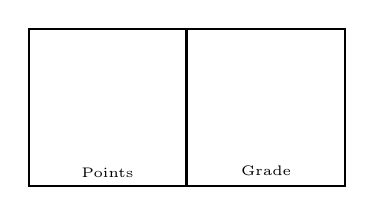
\begin{tikzpicture}[thick]
		\node (points) at (0,0) [draw,minimum size=2cm] {};
		\node (lbl-points) at (points.south) [anchor=south,font=\tiny] {Points};
		\node (grade) at (points.east) [draw,minimum size=2cm,anchor=west,
			outer sep=0] {};
		\node (lbl-grade) at (grade.south) [anchor=south,font=\tiny] {Grade};
	\end{tikzpicture}

	\begin{flushright}

		% Update this with your team number
		%\huge\bfseries
		%Team: XX \\[1em]

		% Update this with your matriculation number, first name, second name
		\large
		Philipp Lehninger 1327039	\\
		Benedikt Morgenbesser 1027440\\
		
	
	\end{flushright}

	\vspace{5em}

	\begin{center}
		{\huge Digital Integrated Circuits Lab (LDIS)}\\[1em]
		{\Large 384.088, Summer Term 2019} \\[2em]
		{\large Supervisors:\\[.5em]
			Christian Krieg, David Radakovits, Axel Jantsch} \\[10em]

		{\Huge Task 3: Documentation}\\[2em]
		{\Huge Amba Thermometer Nexys 4 DDR} \\[10em]
	\end{center}


%	\begin{abstract}
%
%		Enter the abstract of your report here. An abstract summarizes your
%		entire work (i.e., problem statement, motivation, methodology, key
%		findings). It is a good strategy to write a first version of the abstract
%		when you start to work on your report. This gives you a good guideline
%		what to	put and what not to put into the report. Ideally, you re-write
%		the abstract once you finished your report, because only at this point
%		you have all the information available to create a good abstract.
%
%	\end{abstract}

\end{titlepage}
%
%----------------------------------------------------------------------------
%
\fancyhead{}
\rhead[]{\copyright 2019, Benedikt Morgenbesser, Philipp Lehninger @ Vienna University of Technology.}

\section{Introduction}


The \textit{Amba Thermometer Nexys 4 DDR} core reads in data from the temperature sensor on the Nexys 4 DDR board, processes this data in a moving average algorithm and ouputs the temperature on the LED display. The components of the core communicate via the AMBA ABP bus.
\newline
This documentation gives an overview of the system. All subcores are described in their respective chapters, where valuable information for the usage is given and potential problems are highlighted.


\section{System Overview}

A blockdiagram of the system is shown in figure \ref{fig:block}. The core includes general AMBA ABP bus master and slave modules. The sub-components \textit{SensorSlave}, \textit{InputSlave}, \textit{DSPSlave} and \textit{OutputSlave} include an instance of the slave module. The top level design \textit{thermometer} controls the bus via the master module. 
\newline
\newline
\begin{figure}[h!]
	\centering
	\includegraphics[width=0.8\textwidth]{blockdiagram}
	\caption{Block diagram of the thermometer cores with APB Bus communication}
	\label{fig:block}
\end{figure}

\section{AMBA APB Bus}
The communication via the bus is implemented according to the AMBA 3 ABP Protocol v1.0 Specification\footnote{\url{https://static.docs.arm.com/ihi0024/b/AMBA3apb.pdf}}. Please read this specification for further information.

\subsection{ambaMaster}

The \textit{ambaMaster} module operates through the four following states.

\begin{enumerate}
	\item{\textbf{IDLE}} Default state of the module. When a transfer is required the master moves to the SETUP state.
	\item{\textbf{SETUP}} The master asserts the PSELx signal to select one slave. This state remains for only one clock cycle and is followed by the ACCESS state.
	\item{\textbf{ACCESS}} The PENABLE signal is asserted and the read/write access is granted. A transition from this state is controlled by the PREADY signal with following possibilities:
		\subitem After a read access the next state is PROVIDE
		\subitem Else, if another transfer is required, the next state is SETUP
		\subitem If nothing of the above applies the next state is IDLE
	\item{\textbf{PROVIDE}} For a read access the buffered data is provided. Depending on whether there is another transfer requested the follwing state is either IDLE or again SETUP.
\end{enumerate}

The interface of the \textit{ambaMaster} module is shown in figure \ref{fig:ambaMaster}. The interface to the APB bus is according to the AMBA 3 ABP Protocol v1.0 Specification.\footnote{\url{https://static.docs.arm.com/ihi0024/b/AMBA3apb.pdf}} For information about the signals please read the descriptions in this specification. The interface for the communication with the top level design includes the following signals:

\begin{enumerate}
	\item{\textbf{data}} Is a bi-directional 32 bit vector for the communication between top level design und bus master. 
	\item{\textbf{slaveaddr}} A slave is addressed by asserting the respective place in the slave address vector.
	\item{\textbf{regaddr}} Is equivalent to PADDR and not used in this core. It would be only necessary to address registers, if the data exceeds the 32 bit width of the ABP bus.
	\item{\textbf{transferRequest}} Indicates if a transfer is requested.
	\item{\textbf{write}} Indicates an write access if high and a read access if low.
	\item{\textbf{ready}} Indicates if the master module is ready to start a new access if high.
\end{enumerate}
\textbf{Please notice:} If any changes affecting the data signal are applied, make sure to keep consistent with the tristate logic.
\begin{figure}[h!]
	\centering
	\includegraphics[width=0.5\textwidth]{ambaMaster}
	\caption{Interface of the ambaMaster module.}
	\label{fig:ambaMaster}
\end{figure}

\subsection{ambaSlave}
The ambaSlave module generates its current state from the received signals. The interface of the \textit{ambaSlave} module is shown in figure \ref{fig:ambaSlave}.The interfaceto the APB bus is again according to the specification. The interface to the slave modules includes the following signals.
\begin{enumerate}
	\item{\textbf{data_in}} Is a 32 bit vector for the data to be read by the master. 
	\item{\textbf{data_out}} Is a 32 bit vector for the data written by the master.
	\item{\textbf{addr}} Is equivalent to PADDR and not used in this core. It would be only necessary to address registers, if the data exceeds the 32 bit width of the ABP bus.
	\item{\textbf{readreg}} Indicates a read access if high.
	\item{\textbf{writereg}} Indicates a write access if high.
	\item{\textbf{done}} Indicates if the slave finished its operations and a new transfer can be requested.
\end{enumerate}
\textbf{Please notice:} In contrast to the master module the communication for read/write between the slave module and their sub-components is seperated, i.e. an uni-directional bit vector is used for each operation.
\begin{figure}[h!]
	\centering
	\includegraphics[width=0.5\textwidth]{ambaSlave}
	\caption{Interface of the ambaSlave module.}
	\label{fig:ambaSlave}
\end{figure}

\section{thermometer}

Thermometer is the top level entity and controls the bus master via a state machine with the 6 following sequential states:
\begin{enumerate}
	\item \textbf{IDLE:} This state is just used as an initial state for the system after power-up or resets.
	\item \textbf{INPUT:} The user input for the size of the averaging window is read from the Input Module.
	\item \textbf{SENSOR:} The 16 bit 2's complement vector from the Sampling Module is read.
	\item \textbf{FEEDMAVG:} The temperature value and window size are concatenated and written to the Moving Average Module.
	\item \textbf{MAVG:} The averaged temperature is read.
	\item \textbf{OUTPUT:} The averaged temperature vector is written to the Output Module. This state is followed by the INPUT state.
\end{enumerate}
\textbf{Please notice:} A state transition only occurs when the \textit{ready} flag is set by the bus master (Except for the IDLE state).\newline

\subsection{clkdivide}
All clocks are generated in the thermometer module.
\begin{enumerate}
	\item The ABP bus clock is set to 25\,MHz.
	\item The display clock is set to 1\,kHz. (For a cycle of 8 digits, this gives a refresh frequency of 125\,Hz for each digit).
	\item The sample rate is set to 250\,ms per default. This can be adjusted presynthesis according to table \ref{tab:sampling}
\end{enumerate}


\begin{table}[H]
\begin{center}
\begin{tabular}{|c|c|}

\hline
sampling rate value & corresponding sample time \\
\hline
1 & 0.25 sec \\
2 & 0.5 sec \\
4 & 1 sec \\
3 & not valid \\
\hline

\end{tabular}
\caption{Sampling time.}
\label{tab:sampling}
\end{center}
\end{table}

\subsection{AmbaDemux4}
All slaves have to share the PRDATA and PREADY port of the \textit{ambaMaster} module. In order to read from the slaves the \textit{AmbaDemux4} module demultiplexes these signals.

\section{SensorSlave}
The \textit{SensorSlave} module reads data from the \textit{temperature_2comp} register with a sampling rate of 250\,ms, 500\,ms or 1\,s. The sampling rate can be set presynthesis in the \textit{thermometer} module.
\subsection{TempSensorCtl}
The \textit{TempSensorCtl} module is from the Nexsys Demo Version and intellectual property of Elod Gyorgy\footnote{https://github.com/Digilent/Nexys-Video-OLED/releases}. The module reads continiously from the ADT7420 temperature sensor on the board and writes the data to the \textit{temperature_2comp} register. The interface between the sensor and the FPGA is shown in figure \ref{fig:sensor}.

\begin{figure}[h!]
	\centering
	\includegraphics[width=0.5\textwidth]{tempsens}
	\caption{Temperature sensor interface.}
	\label{fig:sensor}
\end{figure}

For the correct implementation of the \textit{TempSensorCtl} module in this core the resolution lenght of the temperature vector was adapted to 16 bit. Therefore, the configuration register (address 0x03) was set to 0x80.

\section{InputSlave}
The \textit{InputSlave} connects the up and down button (BTN_U \& BTN_D) from the Nexsys 4 DDR board to adjust the window size of the moving average algorithm during run time.
\subsection{windowsize}
The \textit{windowsize} module permits four different window sizes, i.e. 1\,x / 2\,x / 4\,x / 8\,x the sampling period.


\section{DSPSlave}
The \textit{DSPSlave} module reads from the master (bits 0-15: temperature data in 2's complement, bits 16-17: windowsize) ,processes it, and writes the averaged temperature back.
\subsection{moving_average}
The \textit{moving_average} module is averaging the temperature according to the window size. For each new writing access, the temperature registers are shifted and the new value is safed in \textit{temp_in_ex0}. To keep the 2's complement addition consistent the MSB is copied to three addtional bits. The division of the summed value is done by shifting.\\
\textbf{Please notice:} Therefore only windowsizes of 2$^n$\,x sampling rates are feasable.



\section{OutputSlave}

\subsection{parsing7seg}
To display the temperature the 2's complement std_logic_vector is converted into an array, where each component represents one digit of the display. One LSB of the temperature sensor is equivalent to 0.0078\,°C. The module first sets a signbit. Then the 2's complement vector is converted to an integer and multiplied by 78. This value represents now the temperature $\cdot$ 1E4. To get the individual digits, the value is divided by the highest decimal power and saved as an integer into the array. This integer times the decimal power is substracted from the original value to get rid of the digit and the process is repeated for the next smaller decimal power...

\subsection{whole7segment}
The eight digits of the display have a common anode and individual cathodes to drive the seven segments. (See figure \ref{7segdigit}.) The digits are addressed periodically.

\begin{figure}[H]
\centering
\includegraphics[width=0.5\textwidth]{7segdigit}
\caption{Eight-digit Seven Segment Display}
\label{7segdigit}
\end{figure}

\end{document}
%
%----------------------------------------------------------------------------

